\documentclass[11pt,a4paper]{article}
\usepackage{amsmath}
\usepackage{amssymb}
\usepackage{amsthm}
\usepackage[utf8]{inputenc}
\usepackage{graphicx}

\usepackage[utf8]{inputenc}
\usepackage[english]{babel}
\usepackage{booktabs}
\usepackage{cite}


\newtheorem{theorem}{Theorem}

\usepackage{listings}
\usepackage{color} %red, green, blue, yellow, cyan, magenta, black, white
\definecolor{mygreen}{RGB}{28,172,0} % color values Red, Green, Blue
\definecolor{mylilas}{RGB}{170,55,241}


\usepackage{graphicx}

\title{Optimization}


\begin{document}
\section{Steepest descent}
The steepest descent method is a very simple line search method that is defined by the following iteration:
\begin{align*}
x^{k+1} = x^k - \alpha\nabla J(x^k)
\end{align*}
If we want to use this method to solve a timedecomposed problem using penalty terms, we would get the following:
\begin{align*}
(v^{k+1},\lambda^{k+1})= (v^k,\lambda^k)-\alpha\nabla J(v^k,\lambda^k)
\end{align*}
One problem with the steepest descent method, is that it is sensitive to bad scaling, and in many cases the size of the gradient with respect to $v$ and $\lambda$ may have a difference of several orders of magnitude. This would result in extremely slow convergence. One way of handling this is to split up the update:
\begin{align*}
v^{k+1} &= v^k - \alpha\nabla J(v^k)\\
\lambda^{k+1} &= \lambda^k - \alpha\nabla J(\lambda^k)
\end{align*}
To illustrate that we have scaling issues, lets look at the DE constrained optimal control problem that we have looked at previously:
\begin{align}
	\left\{
     \begin{array}{lr}
		\frac{\partial y}{\partial t}(t)+Ay=Bv  \ \textit{For $t \in [0,T]$}\\
		y(0)=y^0
	\end{array}
	\right. \label{OC_PDE}
\end{align}
The functional they use is on the following form:
\begin{align}
J(v) = \frac{1}{2}\int_0^T ||v(t)||^2 dt + \frac{\alpha}{2}||y(T)-y^T||^2 \label{OC_func}
\end{align}
This problem yields the following gradient:
\begin{align}
\langle\hat{J}'(v,\lambda),(s,l) \rangle = \int_0^T (B^*p+v)sdt + \sum_{n=1}^{N-1}(p_n(T_n) - p_{n-1}(T_n))l_n \label{penalty grad}
\end{align}
In a numerical setting, where we have discretized the equation, we will get the following gradient:
\begin{align*}
\nabla J(\bar{v},\Lambda) = (\Delta t (v_0-B^*p_0),...,\Delta t (v_{M}-B^*p_M),\{p_n(T_n) - p_{n-1}(T_n)\})
\end{align*}
One sees that the adjoint appears in both parts of the gradient, but in the $v$ part there is a factor of $\Delta t$ multiplied with it. It therefore makes sense, that the there is a factor of $\Delta t$ order of magnitude difference between the size of $v$ and $\Lambda$ part of the gradient. This means that for small $\Delta t$ the steepest descent method will converge very slowly.
\section{Scaling}
An alternative way of handling an unbalanced gradient is to rescale the problem. Lets explain with a simple example, where we try to minimize a function with only two variables $J(x,y)$. We then pick some initial point $(m_1,m_2)$, and notice that the gradient $\nabla J(m_1,m_2)$ is very unbalanced. Ideally, we would want $J_x(m_1)=J_y(m_2)$, and to achieve this we introduce a new functional $\hat{J}(x,\xi)=J(x,\gamma\xi)$, with 
\begin{align*}
\gamma = \frac{\frac{\partial J(m_1,m_2)}{\partial x}}{\frac{\partial J(m_1,m_2)}{\partial y}}
\end{align*} 
Now choose a new initial point $(m_1,\frac{m_2}{\gamma})$, and we see that 
\begin{align*}
\frac{\partial \hat{J}(m_1,\frac{m_2}{\gamma})}{\partial x}=\frac{\partial\hat{J}(m_1,\frac{m_2}{\gamma})}{\partial y}
\end{align*}
because
\begin{align*}
\frac{\partial \hat{J}(m_1,\frac{m_2}{\gamma})}{\partial x} = \frac{\partial J(m_1,m_2)}{\partial x}
\end{align*}
and
\begin{align*}
\frac{\partial\hat{J}(m_1,\frac{m_2}{\gamma})}{\partial y} & = \frac{\partial J(m_1,m_2)}{\partial y}\gamma \\
&=\frac{\partial J(m_1,m_2)}{\partial x}
\end{align*}
\section{Scaling for Steepest descent}
To illustrate how scaling of the time-decomposed problem affects the performance of the steepest descent method, lets look at a simple ODE example of problem (\ref{OC_PDE}-\ref{OC_func}), with parameters $(A,B,T,\alpha,y_0,y_T,\Delta t)=(0.9,1,1,0.5,1.2,5,\frac{1}{500})$. Solving this problem using penalty term $\mu=1$ and different time-decompositions yielded the following:
\\
\begin{tabular}{llllrr}
\toprule
{}decompositions &     $\gamma$ & scaled error & scaled iterations &  error &  iterations \\
\midrule
0  &        -- &           -- &                -- &        0.000000 &                   34 \\
2  &  0.027027 &     0.224357 &                21 &        0.275448 &                  601 \\
4  &      0.04 &     0.425371 &                32 &        0.553890 &                  601 \\
8  &      0.04 &     0.551151 &                79 &        0.609155 &                  601 \\
16 &      0.04 &     0.620472 &               219 &        0.659912 &                  460 \\
32 &      0.04 &     0.657101 &               555 &        0.674689 &                  601 \\
\bottomrule
\end{tabular}
From the table above it is clear that scaling has a huge impact on the performance of the steepest descent algorithm for the time-decomposed problem. Another thing of note is the value of the scaling factor $\gamma$. Since the functional have more than two arguments, we need to choose a way to determine $\gamma$. For the example above, I have used the following:
\begin{align*}
\gamma = 20\frac{||\nabla J(v)||_{\infty}}{||\nabla J(\Lambda)||_{\infty}}
\end{align*} 
One can choose a different factor than twenty to multiply with the fraction, what factor to choose is not obvious. Below I have tested the same problem for different time-decompositions $m$, using different factors to calculate $\gamma$. The resulyts were the following:
\\
\begin{tabular}{lllll}
\toprule
{} & m=16 (iter,$\gamma$) &         m=2 (iter,$\gamma$) & m=4 (iter,$\gamma$) & m=8 (iter,$\gamma$) \\
\midrule
1   &      (501, 0.002) &  (501, 0.00135135135135) &     (501, 0.002) &     (501, 0.002) \\
5   &       (501, 0.01) &   (99, 0.00675675675676) &       (83, 0.01) &      (241, 0.01) \\
10  &       (196, 0.02) &    (30, 0.0135135135135) &       (32, 0.02) &       (80, 0.02) \\
15  &       (188, 0.03) &    (32, 0.0202702702703) &       (40, 0.03) &       (67, 0.03) \\
20  &       (219, 0.04) &     (21, 0.027027027027) &       (32, 0.04) &       (79, 0.04) \\
30  &       (174, 0.06) &    (42, 0.0405405405405) &       (45, 0.06) &       (73, 0.06) \\
50  &        (155, 0.1) &    (28, 0.0675675675676) &        (32, 0.1) &        (65, 0.1) \\
100 &        (155, 0.2) &     (29, 0.135135135135) &        (47, 0.2) &        (84, 0.2) \\
\bottomrule
\end{tabular}
It could also be interesting to look at what happens when we decrease $\Delta t$. I have therefore looked at at the performance of different $\gamma$ values for different mesh sizes, for the problem above decomposed into for time intervals. This gave me the following:
\\
\begin{tabular}{llllll}
\toprule
{} & N=100(itr,$\gamma$,err) & N=200(itr,$\gamma$,err) & N=800(itr,$\gamma$,err) & N=1000(itr,$\gamma$,err) & N=2000(itr,$\gamma$,err) \\
\midrule
 &               (41, --) &               (16, --) &               (11, --) &                (13, --) &                (20, --) \\
1        &       (101, 0.01, 0.6) &      (101, 0.005, 1.2) &    (101, 0.00125, 1.4) &       (101, 0.001, 1.4) &      (101, 0.0005, 1.4) \\
10       &         (26, 0.1, 0.4) &        (26, 0.05, 0.4) &      (63, 0.0125, 0.4) &         (71, 0.01, 0.4) &        (65, 0.005, 0.4) \\
15       &        (48, 0.15, 0.4) &       (39, 0.075, 0.4) &     (31, 0.01875, 0.4) &        (43, 0.015, 0.4) &       (41, 0.0075, 0.4) \\
20       &         (37, 0.2, 0.4) &         (25, 0.1, 0.4) &       (22, 0.025, 0.4) &         (26, 0.02, 0.4) &         (26, 0.01, 0.4) \\
50       &         (83, 0.5, 0.4) &        (64, 0.25, 0.4) &      (24, 0.0625, 0.4) &         (24, 0.05, 0.4) &        (18, 0.025, 0.4) \\
100      &        (101, 1.0, 0.6) &        (101, 0.5, 0.5) &       (39, 0.125, 0.4) &          (29, 0.1, 0.4) &         (26, 0.05, 0.4) \\
\bottomrule
\end{tabular}
\section{L-BFGS}
As with steepest descent the L-BFGS should also be sensitive to scaling. Solving the same optimal control problem as I did for steepest descent, i.e. problem (\ref{OC_PDE}-\ref{OC_func}), with parameters $(A,B,T,\alpha,y_0,y_T,\mu,\Delta t)=(0.9,1,1,0.5,1.2,5,1,\frac{1}{500})$, I tried the scaling technique on L-BFGS for different memory-size using five decomposed time intervals. This yielded the following:
\\
\begin{tabular}{lrrlrr}
\toprule
{} memory length &  scaled err &  scaled itr & steepest descent &  unscaled err &  unscaled itr \\
\midrule
0  &    0.492563 &          41 &               41 &      0.591079 &           501 \\
1  &    0.753307 &         501 &               -- &      0.495369 &            39 \\
5  &    0.492315 &         278 &               -- &      0.491279 &            16 \\
10 &    0.487367 &          95 &               -- &      0.491595 &            17 \\
\bottomrule
\end{tabular} 
 \begin{figure}
  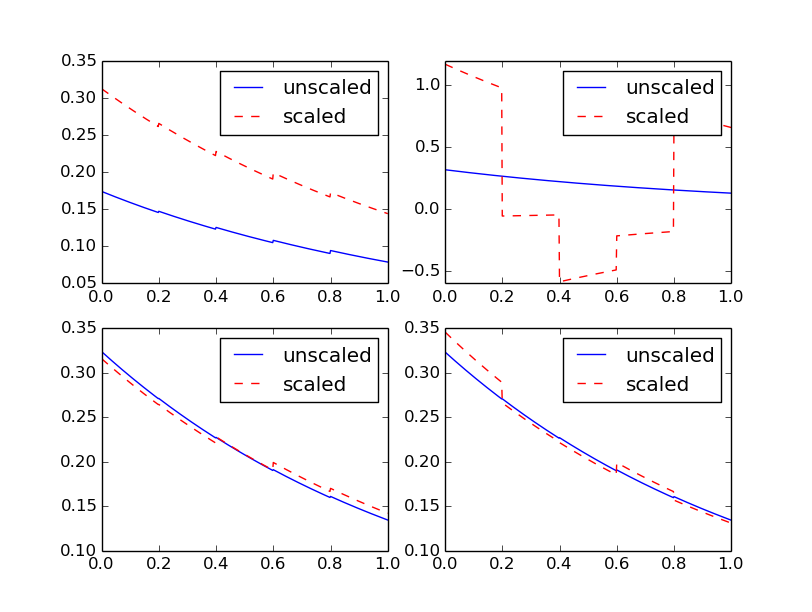
\includegraphics[width=\linewidth]{scale_mem_lim.png}
  \caption{The resulting controls of the scaled and unscaled L-BFGS solution of problem (\ref{OC_PDE}-\ref{OC_func}) using different memory size.} 
  \label{Fig 1}
\end{figure}
The most important note to this result, is that the scaling factor $\gamma$ was set to be 
\begin{align*}
\gamma = 20\frac{||\nabla J(v)||_{\infty}}{||\nabla J(\Lambda)||_{\infty}}=0.04
\end{align*}
This choice worked fine for steepest decent, but as we see from the table, the performance of the L-BFGS worsened when scaled. Also, by error I mean the $L^2$ difference between the control of the penalty solutions, and the control of the non-penalty solution. We notice that the scaled and unscaled methods results in approximately the same error, however by looking at the plots, we see that the controls from the scaled method have more noticeable jumps.
\\
\\
I Then look at what happens when you try to change your scaling parameter $\gamma$. I solve the same problem as before, but now only for memory of length 1. This resulted in the following:
\\
\begin{tabular}{lrrr}
\toprule
{} &  scaled gamma &  scaled iter &  unscaled iter \\
\midrule
1      &         0.002 &          101 &             39 \\
10     &         0.020 &          101 &             39 \\
20     &         0.040 &          101 &             39 \\
100    &         0.200 &          101 &             39 \\
200    &         0.400 &           63 &             39 \\
500    &         1.000 &           39 &             39 \\
1000   &         2.000 &           39 &             39 \\
2000   &         4.000 &           17 &             39 \\
4000   &         8.000 &           21 &             39 \\
10000  &        20.000 &           24 &             39 \\
20000  &        40.000 &           26 &             39 \\
50000  &       100.000 &           28 &             39 \\
100000 &       200.000 &           29 &             39 \\
\bottomrule
\end{tabular}
\section{Scaling the inverse Hessian}
The results of scaling the gradient and using L-BFGS yielded unexpected results. It might therefore be a good idea, to investigate if we also have to change the approximation of the inverse Hessian, and not only the gradient. Lets again return to our simple two-variable example functional $J(x,y)$, and our scaled version of it $\hat{J}(x,\xi)=J(x,\gamma\xi)$. We found the gradient of $\hat{J}$ to be:
\begin{align*}
\nabla \hat{J}(x,\gamma\xi) = (J_x(x,\gamma\xi),\gamma J_y(x,\gamma\xi))
\end{align*}
Finding the Hessian of $\hat{J}$ is also quite simple, and it looks like this:
\begin{align}
  \nabla^2 \hat{J}=\left[ \begin{array}{cc}
   J_{xx} & \gamma J_{xy}\\
    \gamma J_{xy}& \gamma^2J_{yy}\\
   \end{array}  \right]  \label{scaled_hessian}  
\end{align}
Now look at the L-BFGS iteration, which looks like the following:
\begin{align*}
(x^{k+1},y^{k+1}) = (x^k,y^k) - \alpha H_k \nabla J(x^k,y^k)
\end{align*}
Here H is an approximation of the inverse Hessian $ \nabla^2 J^{-1}$. If we scale the problem, we would instead get the update:
\begin{align*}
(x^{k+1},\xi^{k+1}) = (x^k,\xi^k) - \alpha \hat{H_k} \nabla \hat{J}(x^k,\xi^k)
\end{align*}
One would now expect a similar relation between $H_k$ and $\hat{H_k}$ as the one in (\ref{scaled_hessian}) between $\nabla^2 J$ and $\nabla^2 \hat{J}$, only inverted, i.e if $H^k$ was given by
\begin{align*}
	H^k=\left[ \begin{array}{cc}
   	c_1 & c_2\\
    	c_3& c_4\\
   \end{array}  \right]
\end{align*}
We want  $\hat{H_k}$ to be:
\begin{align}
	\hat{H_k}=\left[ \begin{array}{cc}
   	c_1 & \frac{c_2}{\gamma}\\
    	\frac{c_3}{\gamma}& \frac{c_4}{\gamma^2}\\
   \end{array}  \right] \label{Ihessian_property}
\end{align}
With this observation in mind, lets now take a closer look at the L-BFGS inverse Hessian approximation, to see if the above statement actually holds. To make it simple I will only consider the case where we use L-BFGS with memory length 1. First lets remember how the L-BFGS inverse Hessian approximation update looks like:
\begin{align*}
H^{k+1} &= (I-\rho_kS_kY_k^T)H^k(I-\rho_kY_kS_k^T) + S_kS_k^T\\
S_k &= x^{k+1}-x^{k} \\
Y_k &= \nabla J(x^{k+1})-\nabla J(x^{k})\\
\rho_k &= \frac{1}{Y_k^TS_k} \\
H^0 &= \beta I
\end{align*}
Lets find the $H_k$ in the case where we only use information of the last iteration in the update, and where we solve a two variable problem. Define $S_k=[a,b]^T$ and $Y_k=[x,y]^T$. The algebra now becomes quite ugly, so its best to split up the derivation:
\begin{align*}
A &= (I-\rho_kS_kY_k^T) \\
&=\left[ \begin{array}{cc}
   	1-\rho ax & -\rho ay\\
    	-\rho bx& 1-\rho by\\
   \end{array}  \right] \\
&=\left[ \begin{array}{cc}
   	1-d_1 & -d_2\\
    	-d_3& 1-d_4\\
   \end{array}  \right] \\
B &= (I-\rho_kS_kY_k^T)I(I-\rho_kY_kS_k^T) = AA^T \\
&=\left[ \begin{array}{cc}
   	(1-d_1)^2 + d_2^2& -d_3(1-d_1) -d_2(1-d_4)\\
    	-d_3(1-c1)-d_2(1-d_4)& (1-d_4)^2 +d_3^2\\
   \end{array}  \right] \\
C&= \rho S_kS_k^T \\
&=\rho\left[ \begin{array}{cc}
   	a^2  & ab\\
    	ab& b^2\\
   \end{array}  \right] \\
H^{k+1}&=B+C
\end{align*}
Now lets find the scaled inverted Hessian. The first thing to notice, is that both the $S_k$ and $Y_k$ changes, since you multiply the the second part of the gradient with $\gamma$, while you divide the second variable with $\gamma$. this results in $\hat{S}_k=[a,\frac{b}{\gamma}]^T$ and $\hat{Y}_k=[x,\gamma Y]^T$. Notice that that means that $\rho$ stays unchanged. Now lets derive $\hat{H}^{k+1}$:
\begin{align*}
\hat{A} &= (I-\rho_k\hat{S}_k\hat{Y}_k^T) \\
&=\left[ \begin{array}{cc}
   	1-\rho ax & -\rho ay\gamma\\
    	-\rho \frac{bx}{\gamma}& 1-\rho by\\
   \end{array}  \right] \\
&=\left[ \begin{array}{cc}
   	1-d_1 & -d_2\gamma\\
    	-\frac{d_3}{\gamma}& 1-d_4\\
   \end{array}  \right] \\
\hat{B} &= (I-\rho_k\hat{S}_k\hat{Y}_k^T)I(I-\rho_k\hat{Y}_k\hat{S}_k^T) = \hat{A}\hat{A}^T \\
&=\left[ \begin{array}{cc}
   	(1-d_1)^2 + (d_2\gamma)^2& -\frac{d_3}{\gamma}(1-d_1) -d_2\gamma(1-d_4)\\
    	-\frac{d_3}{\gamma}(1-c1)-d_2\gamma(1-d_4)& (1-d_4)^2 +(\frac{d_3}{\gamma})^2\\
   \end{array}  \right] \\
\hat{C}&= \rho \hat{S}_k\hat{S}_k^T \\
&=\rho\left[ \begin{array}{cc}
   	a^2  & \frac{ab}{\gamma}\\
    	\frac{ab}{\gamma}& (\frac{b}{\gamma})^2\\
   \end{array}  \right] \\
\hat{H}^{k+1}&=\hat{B}+\hat{C}
\end{align*}
The impotent thing to note about the above derivation, is that we almost, but not quite get the property (\ref{Ihessian_property}). The problem arises in $\hat{B}$, where multiple terms have the wrong factor of $\gamma$ multiplied with them. However, it turns out that this can be fixed by a slight change to to the formula, namely changing $H^0=I$, to:
\begin{align*}
	H^0 = \left[ \begin{array}{cc}
   	1 & 0\\
    	0& \frac{1}{\gamma^2}\\
   \end{array}  \right]
\end{align*}
This would then give us 
\begin{align*}
\hat{B} &= (I-\rho_k\hat{S}_k\hat{Y}_k^T)H^0(I-\rho_k\hat{Y}_k\hat{S}_k^T)  \\
&=\left[ \begin{array}{cc}
   	(1-d_1)^2 + d_2^2& -\frac{d_3}{\gamma}(1-d_1) -\frac{d_2}{\gamma}(1-d_4)\\
    	-\frac{d_3}{\gamma}(1-c1)-\frac{d_2}{\gamma}(1-d_4)& (\frac{1-d_4}{\gamma})^2 +(\frac{d_3}{\gamma})^2\\
   \end{array}  \right] \\
\end{align*}
Now $\hat{H}^{k+1}=\hat{B}+\hat{C}$ will satisfy (\ref{Ihessian_property}). The next step to check if the changed initial inverted Hessian have any impact on the performance of the scaled L-BFGS method. I have therefore, with this goal in mind redone the experiments for the scaled L-BFGS, using the same equations and parameters, with the changes proposed above. This yielded the following:
\\
\begin{tabular}{lrrrr}
\toprule
{} memory length &  scaled err &  scaled itr &  unscaled err &  unscaled itr \\
\midrule
1  &    0.146630 &          62 &      0.131932 &            82 \\
2  &    0.126179 &          17 &      0.129110 &            24 \\
5  &    0.127947 &          11 &      0.127947 &            11 \\
10 &    0.128153 &           8 &      0.129299 &             9 \\
\bottomrule
\end{tabular}
\\
While L-BFGS without a scaled $H^0$ required a lot more iterations, to reach its tolerance, the L-BFGS with scaled $H^0$ performs either better or as good as the unscaled version. For this example we used the same $\gamma$ as before, namely:
\begin{align*}
\gamma = 20\frac{||\nabla J(v)||_{\infty}}{||\nabla J(\Lambda)||_{\infty}}
\end{align*}
It might therefore be interesting to see what value of $\gamma$ that is optimal for L-BFGS with scaled $H^0$. The result for a repetition of the changing $\gamma$ experiment for L-BFGS using memory length 1 follows below:
\\
\begin{tabular}{lrrr}
\toprule
{} &  scaled gamma &  scaled iter &  unscaled iter \\
\midrule
0.25     &        0.0005 &           30 &             39 \\
0.50     &        0.0010 &           30 &             39 \\
0.75     &        0.0015 &           30 &             39 \\
1.00     &        0.0020 &           30 &             39 \\
10.00    &        0.0200 &           34 &             39 \\
20.00    &        0.0400 &           34 &             39 \\
100.00   &        0.2000 &           38 &             39 \\
200.00   &        0.4000 &           38 &             39 \\
500.00   &        1.0000 &           39 &             39 \\
1000.00  &        2.0000 &           39 &             39 \\
2000.00  &        4.0000 &           39 &             39 \\
20000.00 &       40.0000 &           39 &             39 \\
50000.00 &      100.0000 &           51 &             39 \\
\bottomrule
\end{tabular}
\\
The important findings in the previous experiment, is that choosing $\gamma$ to be 
\begin{align*}
\gamma = \frac{||\nabla J(v)||_{\infty}}{||\nabla J(\Lambda)||_{\infty}}
\end{align*}
actually works best. This is also what one would intuitively expect.  
\end{document}